%Este trabalho está licenciado sob a Licença Creative Commons Atribuição-CompartilhaIgual 3.0 Não Adaptada. Para ver uma cópia desta licença, visite https://creativecommons.org/licenses/by-sa/3.0/ ou envie uma carta para Creative Commons, PO Box 1866, Mountain View, CA 94042, USA.
% !TEX root = ../main.tex

\chapter{Campos vetoriais}\label{cap:campos}\index{campos vetoriais}


\section{Campos escalares e campos vetoriais}
 Campo é termo usado para designar funções definidas em uma porção do espaço tridimensional (ou bidimensional), isto é, funções cujo domínio $D$ é um subconjunto de $\mathbb{R}^3$ (ou $\mathbb{R}^2$). Trabalharemos com dois tipos de campos: os campos escalares e os campos vetoriais. Os campos vetoriais são funções cuja imagem é composta de vetores no $\mathbb{R}^3$, já a imagem dos campos escalares são números reais, isto é, escalares.

\begin{ex}\label{excampos} São exemplos de campos escalares.
\begin{itemize}
\item [a)] A função que liga a posição de um ponto dentro de uma sala à temperatura neste ponto.
\item [b)] A pressão do ar como função da posição na atmosfera.
\item [c)] $f(x,y,z)= 100 + 20e^{-\sqrt{x^2+y^2+z^2}}$.
\item [d)] $f(x,y,z)= \vec{r} \cdot \vec{r} = x^2+y^2+z^2$, onde $\vec{r}=x\vec{i}+y\vec{j}+z\vec{k}$ .
\end{itemize}
\end{ex}


\begin{ex}\label{excampos_1} São exemplos de campos vetoriais.
\begin{itemize}
\item [a)] A função que liga a posição de um ponto dentro de uma fluido à velocidade (vetor) neste ponto.
\item [b)] O campo magnéticos, elétrico, gravitacional etc.
\item [c)] $\vec{F}(x,y,z)= x\vec{i} + z\vec{j} - y\vec{k}$.
\item [d)] $\vec{F}(x,y,z)= \vec{r}\times \vec{k}$
\end{itemize}
\end{ex}

\section{Representação gráfica dos campos vetoriais}
Um campo vetorial é representado graficamente por um conjunto de setas partindo de pontos $(x,y,z)$ e de comprimento proporcional ao módulo de $\vec{F}(x,y,z)$ e mesma direção e sentido de $\vec{F}(x,y,z)$. O conjunto de pontos é escolhido de forma arbitrária de forma a permitir interpretar o campo.

\begin{ex} Represente graficamente o campo vetorial $\vec{F}(x,y)=\sqrt{y}\ \!\vec{i},~~y\geq 0$.
%\begin{figure}[htp]
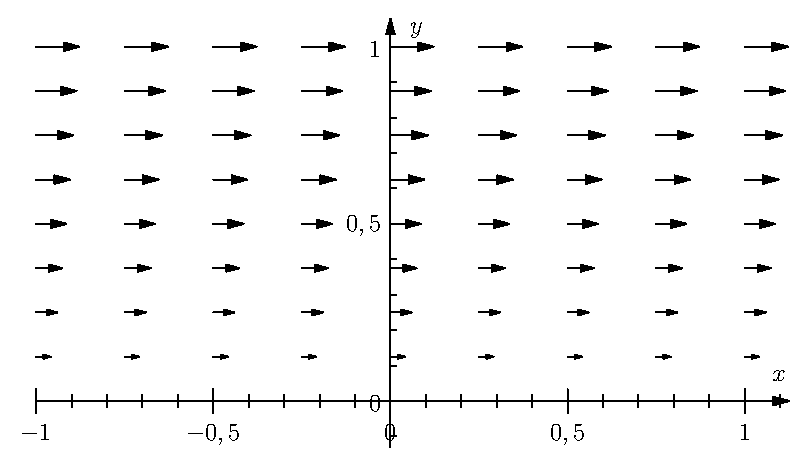
\includegraphics{cap_campos/figs/campo_exemplo_1}
%\caption{\label{campo_radial}Representação gráfica do campo $\vec{F}(x,y)=\sqrt{y}\ \!\vec{i},~~y\geq 0$.}
%\end{figure}
\end{ex}


\begin{ex} Represente graficamente o campo vetorial $\vec{F}(x,y)=x\vec{i},~~y\geq 0$.
%\begin{figure}[htp]
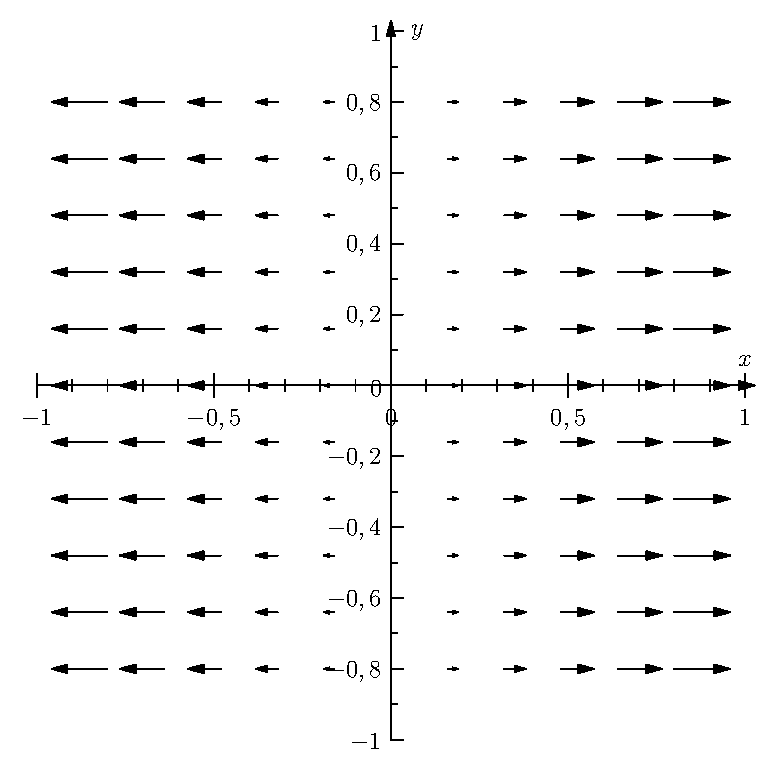
\includegraphics{cap_campos/figs/campo_exemplo_2}
%\caption{\label{campo_radial}Representação gráfica do campo $\vec{F}(x,y)=x\vec{i}$.}
%\end{figure}
\end{ex}

\begin{ex} Represente graficamente o campo vetorial $\vec{F}(x,y)=-y\vec{i}+x\vec{j}$.
%\begin{figure}[htp]
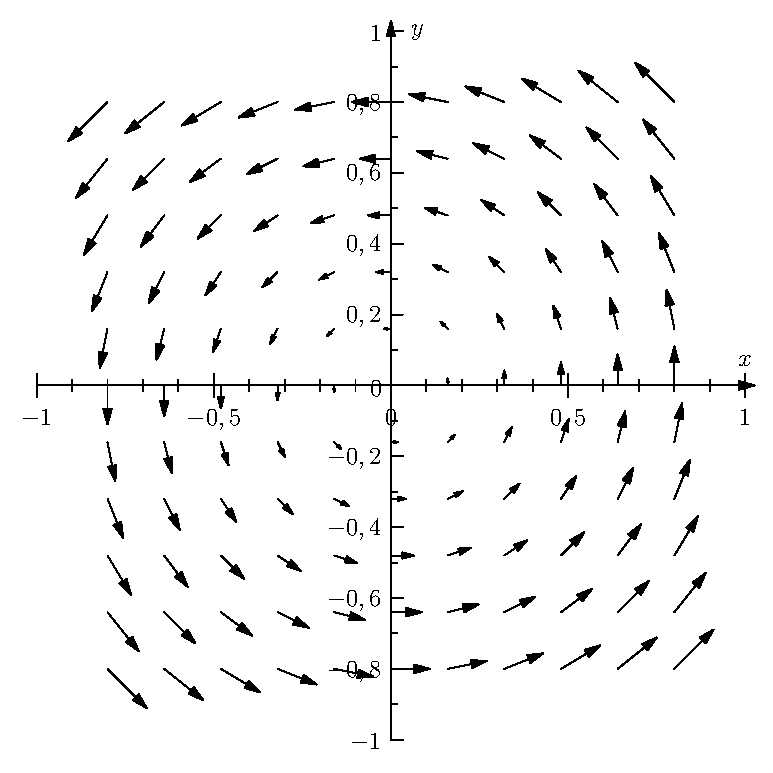
\includegraphics{cap_campos/figs/campo_exemplo_3}
%\caption{\label{campo_radial}Representação gráfica do campo $\vec{F}(x,y)=-y\vec{i}+x\vec{j}$.}
%\end{figure}
\end{ex}

\subsection*{Exercícios}
\begin{exer}
 Faça um esboço dos campos vetoriais $\vec{F}$. Procure representar os vetores com as respectivas proporções:
 \begin{itemize}
  \item[a)] $\vec{F}(x,y)=2\vec{i}-\vec{j}$.
  \item[b)] $\vec{F}(x,y)=y\vec{i}-x\vec{j}$;
  \item[c)] $\vec{F}(x,y)=\frac{1}{\sqrt{x^2+y^2}}\left(x\vec{i}+y\vec{j}\right)$;
 \end{itemize}
\end{exer}


\section{Cálculo com o operador nabla}
\subsection{Definição matemática de divergente, gradiente e rotacional}
No cálculo vetorial, o operador $\vec{\nabla}$, pronunciado nabla ou del, é um símbolo usado para denotar uma série de operadores diferenciais definidos em campos escalares e vetorias, como gradiente, divergente e rotacional. Ele é definido simbolicamente como:
\begin{equation}\label{def_del}
\vec{\nabla} \equiv \vec{i}\frac{\partial}{\partial x}+\vec{j}\frac{\partial}{\partial y}+\vec{k}\frac{\partial}{\partial z}
\end{equation}
Rigorosamente falando, o operador del não é um operador diferencial, mas um mnemônico que ajuda a lembrar de uma série de operadores diferenciais:
\begin{eqnarray*}
 \vec{\nabla}f &=& \vec{i}~\!\frac{\partial f}{\partial x}+\vec{j}~\!\frac{\partial f}{\partial y}+\vec{k}~\!\frac{\partial f}{\partial z} ~~ \text{(Gradiente)},\\
 \vec{\nabla}\cdot \vec{F} &=& \frac{\partial F_1}{\partial x}+\frac{\partial F_2}{\partial y}+\frac{\partial F_3}{\partial z} ~~ \text{(Divergente)},\\
 \vec{\nabla}\times \vec{F} &=&  \vec{i}\left(\frac{\partial F_3}{\partial y}-\frac{\partial F_2}{\partial z}\right) + \vec{j}\left(\frac{\partial F_1}{\partial z}-\frac{\partial F_3}{\partial x}\right) + \vec{k}\left(\frac{\partial F_2}{\partial x}-\frac{\partial F_1}{\partial y}\right)~~ \text{(Rotacional)}.\\
\end{eqnarray*}
O rotacional pode ser representado pelo seguinte determinante simbólico, que funciona como um mnemônico para lembrar facilmente de sua definição:
$$
 \vec{\nabla}\times \vec{F}=\left|
 \begin{array}{ccc}
 \vec{i} & \vec{j} & \vec{k} \\
 \frac{\partial}{\partial x} &\frac{\partial}{\partial y} &\frac{\partial}{\partial z} \\
F_1 & F_2 & F_3
 \end{array}
\right|.
$$

\begin{ex} Calule o gradiente do campo escalar dado por $f(x,y,z)=xy+z$.
\begin{eqnarray}
 \vec{\nabla}f &=& \vec{i}~\!\frac{\partial f}{\partial x}+\vec{j}~\!\frac{\partial f}{\partial y}+\vec{k}~\!\frac{\partial f}{\partial z}
 =y\vec{i}+x\vec{j}+\vec{k}
\end{eqnarray}
\end{ex}

\begin{ex} Calule o divergente e o rotacional do campo vetorial dado por $\vec{F}=(yz+x)\vec{i}+z^2\vec{j}+z^3\vec{k}$.
\begin{eqnarray}
 \vec{\nabla}\cdot \vec{F} &=& \frac{\partial F_1}{\partial x}+\frac{\partial F_2}{\partial y}+\frac{\partial F_3}{\partial z} =
 1+0+3z^2=3z^2+1
\end{eqnarray}

\begin{eqnarray}
  \vec{\nabla}\times \vec{F}&=&\left|
 \begin{array}{ccc}
 \vec{i} & \vec{j} & \vec{k} \\
 \frac{\partial}{\partial x} &\frac{\partial}{\partial y} &\frac{\partial}{\partial z} \\
yz+x & z^2 & z^3
 \end{array}
\right|\\&=&\left(0-2z\right)\vec{i}+\left(y-0\right)\vec{j}+\left(0-z\right)\vec{k}\\
&=&-2z\vec{i}+y\vec{j}-z\vec{k}.
\end{eqnarray}
\end{ex}

\begin{ex} Dado o campo vetorial dado por $\vec{F}=x^5\vec{i}+y^2\vec{j}$, calcule o gradiente do divergente,$ \vec{\nabla} \vec{\nabla}\cdot \vec{F}$, de $\vec{F}$
\begin{eqnarray}
 \vec{\nabla}\cdot \vec{F} &=& \frac{\partial F_1}{\partial x}+\frac{\partial F_2}{\partial y}+\frac{\partial F_3}{\partial z} =
 5x^4+2y\\
 \vec{\nabla} \vec{\nabla}\cdot \vec{F}&=&20x^3\vec{i}+2\vec{j}
\end{eqnarray}
 \end{ex}


\subsection{Operadores diferenciais de segunda ordem}
Operadores diferenciais de segunda ordem podem ser definidos através da composição de operadores diferenciais de segunda ordem. Combinando o gradiente, rotacional e divergente, encontramos as seguintes possibilidades:\index{operador!de segunda ordem}\index{operador!laplaciano}
\begin{eqnarray}
  \vec{\nabla} \cdot \vec{\nabla} f&~& \text{(Divergente do gradiente ou laplaciano)}\\
  \vec{\nabla} \times \vec{\nabla} f&~& \text{(Rotacional do gradiente)}\\
  \vec{\nabla} \vec{\nabla}\cdot \vec{F}&~& \text{(Gradiente do divergente)}\\
  \vec{\nabla} \cdot\vec{\nabla}\times \vec{F}&~& \text{(Divergente do rotacional)}\\
  \vec{\nabla} \times\vec{\nabla}\times \vec{F}&~& \text{(Rotacional do rotacional)}\\
  \end{eqnarray}
As expressões $\vec{\nabla} \times \vec{\nabla} f$ e $\vec{\nabla} \cdot{\nabla}\times \vec{F}$ são identicamente nulas para campos duas vezes continuamente diferenciáveis, o que pode ser provado por simples inspeção:
\begin{eqnarray}
 \vec{\nabla} \times \vec{\nabla} f &=&\left|
 \begin{array}{ccc}
 \vec{i} & \vec{j} & \vec{k} \\
 \frac{\partial}{\partial x} &\frac{\partial}{\partial y} &\frac{\partial}{\partial z} \\
\frac{\partial f}{\partial x} & \frac{\partial f}{\partial y} & \frac{\partial f}{\partial z}
 \end{array}
\right|\\
&=&\vec{i}\left(\frac{\partial^2 f }{\partial z\partial y} - \frac{\partial^2 f}{\partial y\partial z}\right)\\
&+& \vec{j}\left(\frac{\partial^2 f}{\partial  x\partial z}-\frac{\partial^2f}{\partial z\partial x}\right)\\
 &+& \vec{k}\left(\frac{\partial^2 f}{\partial y\partial x}-\frac{\partial^2 f}{\partial x\partial y}\right)
\end{eqnarray}
Sob a regularidade exigida, as derivadas parciais podem ser comutadas e cada termo do rotacional é nulo, isto é:
\begin{eqnarray}
 \vec{\nabla} \cdot \vec{\nabla}\times\vec{F} &\equiv &0
\end{eqnarray}
A demonstração é análoga para o divergente do gradiente.

\subsection{Identidades envolvendo o operador nabla}
Nesta seção, discutimos alguma identidades envolvendo o operador $\vec{\nabla}$. Sejam $f=f(x,y,z)$ e $g=g(x,y,z)$ campos escalares e $\vec{F}=\vec{F}(x,y,z)$ e $\vec{G}=\vec{G}(x,y,z)$ campos vetoriais. Então, valem as identidades da tabela~\ref{tab_identidades_del}.
\begin{table}
 \caption{ Tabela do operador $\vec{\nabla}$} \label{tab_identidades_del}
\begin{tabular}{|l|c|}
\hline
1.& $\displaystyle\vec{\nabla}\left(f+g\right)=\vec{\nabla}f+\vec{\nabla}g$\\
\hline
2.& $\displaystyle\vec{\nabla}\cdot\left(\vec{F}+\vec{G}\right)=\vec{\nabla}\cdot \vec{F}+\vec{\nabla}\cdot \vec{G}$\\
\hline
3.&  $\displaystyle\vec{\nabla}\times\left(\vec{F}+\vec{G}\right)=\vec{\nabla}\times \vec{F}+\vec{\nabla}\times \vec{G}$\\
\hline
4.&  $\displaystyle\vec{\nabla}\left(fg\right)=f\vec{\nabla} g+g\vec{\nabla} f$\\
\hline
5.&  $\displaystyle\vec{\nabla}\cdot\left(f\vec{F}\right)=\left(\vec{\nabla}f\right) \cdot\vec{F}+f\left(\vec{\nabla}\cdot \vec{F}\right)$\\
\hline
6.&   $\displaystyle\vec{\nabla}\times\left(f\vec{F}\right)=\vec{\nabla}f \times\vec{F}+f\vec{\nabla}\times \vec{F}$\\
\hline
7.&  \begin{tabular}{c} $\displaystyle\vec{\nabla}\cdot \vec{\nabla} f=\vec{\nabla}^2f=\frac{\partial^2f}{\partial x^2}+\frac{\partial^2f}{\partial y^2}+\frac{\partial^2f}{\partial z^2}$,\\onde $\vec{\nabla}^2=\frac{\partial^2}{\partial x^2}+\frac{\partial^2}{\partial y^2}+\frac{\partial^2}{\partial z^2}$ é o operador laplaciano	\end{tabular}\\
\hline
8.&$\displaystyle\vec{\nabla}\times\left( \vec{\nabla} f\right)=0$\\
\hline
9.&$\displaystyle\vec{\nabla}\cdot\left( \vec{\nabla}\times \vec{F}\right)=0$\\
\hline
10.&$\displaystyle\vec{\nabla}\times\left( \vec{\nabla}\times \vec{F}\right)=\vec{\nabla}\left(\vec{\nabla}\cdot \vec{F}\right)-\vec{\nabla}^2\vec{F}$\\
\hline
11.&$\displaystyle\vec{\nabla}\cdot\left( \vec{F}\times \vec{G}\right)=G\cdot \left(\vec{\nabla}\times\vec{F}\right)-F\cdot \left(\vec{\nabla}\times\vec{G}\right)$\\
\hline
12.&$\displaystyle\begin{array}{l}\vec{\nabla}\times\left( \vec{F}\times \vec{G}\right)=\left(\vec{G}\cdot \vec{\nabla}\right)\vec{F}-\vec{G}\left(\vec{\nabla}\cdot \vec{F}\right)-\\ ~\qquad\qquad\qquad-\left(\vec{F}\cdot \vec{\nabla}\right)\vec{G}+\vec{F}\left(\vec{\nabla}\cdot \vec{G}\right)\end{array}$\\
\hline
13.&$\displaystyle\begin{array}{l}\vec{\nabla}\left( \vec{F}\cdot \vec{G}\right)=\left(\vec{G}\cdot \vec{\nabla}\right)\vec{F}+\left(\vec{F}\cdot \vec{\nabla}\right)\vec{G}+\\\qquad\qquad\quad+\vec{F}\times\left(\vec{\nabla} \times \vec{G}\right)+\vec{G}\times\left(\vec{\nabla} \times \vec{F}\right)\end{array}$\\
\hline
14.&$\vec{\nabla}\varphi(r) = \varphi'(r)\hat{r}$\\
\hline
\end{tabular}
\end{table}

\subsection*{Exercícios resolvidos}
\begin{exeresol}
  Mostre que $\vec{\nabla}\cdot\left(\vec{\nabla}f \times \vec{\nabla}g\right)=\vec{0}$
\end{exeresol}
\begin{resol}
\begin{eqnarray*}
 E&=&\vec{\nabla}\cdot\left(\vec{\nabla}f \times \vec{\nabla}g\right) \\
  &=&\vec{\nabla}g\cdot\left(\vec{\nabla}\times \vec{\nabla}f\right)+\vec{\nabla}f\cdot\left(\vec{\nabla}\times \vec{\nabla}g\right) ~~~{\color{red} tab(11)~\text{com}~\vec{F}=\nabla f~\text{e}~\vec{G}=\nabla g.}\\
  &=&0~~~{\color{red} tab(8)}\\
\end{eqnarray*}
\end{resol}

\begin{exeresol}
Simplifique $\vec{\nabla}\times\left(\vec{F}\vec{\nabla}\cdot\vec{F}\right)+\vec{F}\times\left[\vec{\nabla}\times\vec{\nabla}\times \vec{F}\right]+\vec{F}\times \vec{\nabla}^2\vec{F}$ e mostre que esta expressão equivale a $(\vec{\nabla}\cdot\vec{F})(\vec{\nabla}\times\vec{F})$
\end{exeresol}
\begin{resol}
\begin{eqnarray*}
 \vec{E}&=&\vec{\nabla}\times\left(\vec{F}\vec{\nabla}\cdot\vec{F}\right)+\vec{F}\times\left[\vec{\nabla}\times\vec{\nabla}\times \vec{F}\right]+\vec{F}\times \vec{\nabla}^2\vec{F}\\
 &=&\vec{\nabla}\times\left(\vec{F}\vec{\nabla}\cdot\vec{F}\right)+\vec{F}\times\left[\vec{\nabla}\times\vec{\nabla}\times \vec{F}+\vec{\nabla}^2\vec{F}\right]\\
 &=&\vec{\nabla}\times\left(\vec{F}\vec{\nabla}\cdot\vec{F}\right)+\vec{F}\times\vec{\nabla}(\vec{\nabla}\cdot\vec{F}) ~~~{\color{red} tab(10)}\\
 &=&\left[\vec{\nabla}(\vec{\nabla}\cdot \vec{F})\times \vec{F}+(\vec{\nabla}\cdot\vec{F})(\vec{\nabla}\times\vec{F})\right]+\vec{F}\times\vec{\nabla}(\vec{\nabla}\cdot\vec{F}),~~~~{\color{red} tab(6)~\text{com}~f=\vec{\nabla}\cdot\vec{F}.}\\
 &=&(\vec{\nabla}\cdot\vec{F})(\vec{\nabla}\times\vec{F})
 \end{eqnarray*}
 Onde se usou que $\vec{A}\times\vec{B}=-\vec{B}\times\vec{A}$.\\
\end{resol}
\begin{exeresol}

Verifique $tab(10)$, isto é, $\vec{\nabla}\times\vec{\nabla}\times \vec{F}=\vec{\nabla}\vec{\nabla}\cdot \vec{F}-\vec{\nabla}^2\vec{F}$ para $$\vec{F}= x^2y\vec{i}+xyz\vec{j}+z^2y\vec{k}.$$
\end{exeresol}
\begin{resol}


 \begin{eqnarray*}
   \vec{\nabla}\times \vec{F}&=&\left|
   \begin{array}{ccc}
    \vec{i}&\vec{j}&\vec{k}\\[.5cm]
    \frac{\partial }{\partial x}&\frac{\partial }{\partial y}&\frac{\partial }{\partial z}\\[.5cm]
    x^2y&xyz&z^2y
   \end{array}\right|\\
   &=&\left(z^2-xy\right)\vec{i}+\left(0-0\right)\vec{j}+\left(yz-x^2\right)\vec{k}
 \end{eqnarray*}

 \begin{eqnarray*}
   \vec{\nabla}\times\vec{\nabla}\times \vec{F}&=&\left|
   \begin{array}{ccc}
    \vec{i}&\vec{j}&\vec{k}\\[.5cm]
    \frac{\partial }{\partial x}&\frac{\partial }{\partial y}&\frac{\partial }{\partial z}\\[.5cm]
    (z^2-xy)&0&(yz-x^2)
   \end{array}\right|\\
   &=&\left(z-0\right)\vec{i}+\left(2z+2x\right)\vec{j}+\left(0+x\right)\vec{k}
 \end{eqnarray*}
 \begin{eqnarray*}
  \vec{\nabla}(\vec{\nabla}\cdot\vec{F})&=&\vec{\nabla}(2xy+xz+2yz)\\
  &=&(2y+z)\vec{i}+(2x+2z)\vec{j}+(x+2y)\vec{k}
 \end{eqnarray*}

\begin{eqnarray*}
  \vec{\nabla}^2\vec{F}&=&2y\vec{i}+0\vec{j}+2y\vec{k}
 \end{eqnarray*}

 Vemos que a identidade se verifica.

\end{resol}

\subsection*{Exercícios}
 \subsection*{Exercícios}
\begin{exer}
 Calcule o divergente e o rotacional do campo $\vec{F}$ para
 \begin{itemize}
  \item[a)] $\vec{F}=x^2\vec{i}-2\vec{j}+yz\vec{k}$
  \item[b)] $\vec{F}=e^{xy}\vec{i}-\cos(y)\vec{j}+\sin^2(z)\vec{k}$ 
 \end{itemize}
\end{exer}
\begin{resp}
 \begin{itemize}
  \item[a)] $\vec{\nabla}\cdot\vec{F}=2x+y$ e $\vec{\nabla}\times \vec{F}=z\vec{i}$
  \item[b)] $\vec{\nabla}\cdot\vec{F}=ye^{xy}+\sin(y)+\sin(2z)$ e $\vec{\nabla}\times \vec{F}=-xe^{xy}\vec{k}$
 \end{itemize}
\end{resp}

\begin{exer}
Mostre que se $\vec{u}=a\vec{i}+b\vec{j}+c\vec{k}$, onde $a$, $b$ e $c$ são constantes, e $\vec{r}=x\vec{i}+y\vec{j}+z\vec{k}$, então:
\begin{itemize}
 \item[a)] $\vec{\nabla}\cdot (\vec{u}\times \vec{r})=0$ .
 \item[b)] $\vec{\nabla}\times (\vec{u}\times \vec{r})=2\vec{u}$.
\end{itemize}
\end{exer}
\begin{exer} Dado $f=2xz^4-x^2y$, calcule $\vec{\nabla}f$ e $\|\vec{\nabla}f\|$ no ponto $P(2,-2,1)$.
\end{exer}
\begin{resp}
 $\vec{\nabla}f=10\vec{i}-4\vec{j}+16\vec{k}$ e $\|\vec{\nabla}f\|=2\sqrt{93}$.
\end{resp}
\begin{exer}
Mostre que $(\vec{F}\cdot\vec{\nabla})\vec{r}=\vec{F}$, onde $\vec{F}=f(x,y,z)\vec{i}+g(x,y,z)\vec{j}+h(x,y,z)\vec{k}$.
\end{exer}

\begin{exer}
 Mostre que
 $$
 \vec{\nabla}^2(fg)=f\vec{\nabla}^2g+2\vec{\nabla}f\cdot \vec{\nabla}g+g\vec{\nabla}^2f.
 $$
\end{exer}
\begin{exer}
 Use a  tabela do operador del para mostrar que:
 \begin{itemize}
  \item[a)] $(\vec{F}\cdot\vec{\nabla})\vec{F}=\frac{1}{2}\vec{\nabla}(\vec{F}\cdot\vec{F})-\vec{F}\times (\vec{\nabla}\times\vec{F})$.
  \item[b)] $\vec{\nabla}\cdot(\vec{F}\times\vec{r})=\vec{r}\cdot(\vec{\nabla}\times\vec{F})$.
 \end{itemize}
\end{exer}


\section{Derivada direcional e gradiente}


\subsection*{Exercícios resolvidos}
\begin{exeresol}
A temperatura da um ponto $P(x, y)$ de uma placa metálica é:
$$T(x, y) = \frac{xy}{1+x^2+y^2}$$
Encontre a taxa de variação da temperatura em $(1, 1)$ na direção do vetor $\vec{a}=2\vec{i}-\vec{j}$.
\end{exeresol}
\begin{resol}
Primeiro normalizamos o vetor $\vec{a}$ para obter o versor com sua direção e sentido:
\begin{eqnarray*}
\vec{u}&=&\frac{\vec{a}}{\|\vec{a}\|}=\frac{2\vec{i}-\vec{j}}{\sqrt{2^2+1^2}}\\
&=&\frac{\sqrt{5}}{5}\left(2\vec{i}-\vec{j}\right).
\end{eqnarray*}
Agora calculamos o gradiente da função dada:
$$\vec{\nabla}T(x, y) = \frac{y(1-x^2+y^2)\vec{i} + x(1+x^2-y^2)\vec{j}}{\left(1+x^2+y^2\right)^2}.$$
Substituimos no ponto $x=y=1$:
$$\vec{\nabla}T(1, 1) = \frac{\vec{i} + \vec{j}}{9}.$$
A derivada direcional é dada por:
$$\vec{u}\cdot\vec{\nabla}T(1,1) = \frac{\sqrt{5}}{5}\left(2\vec{i}-\vec{j}\right)\cdot \frac{\vec{i} + \vec{j}}{9}=\frac{\sqrt{5}}{45}$$
\end{resol}

\section{Equação da continuidade e divergente}
Seção sobre interpretação do divergente..............


\subsection*{Exercícios}
\begin{exer}
Use a equação da continuidade para mostrar que um fluido incompressível e em estado estacionário o campo de velocidade $\vec{v}$ é tal que $\vec{\nabla}\cdot \vec{v}=0$.
\end{exer}
\begin{exer}
 O escoamento de um fluido incompressível e estacionário é regido pelo campo vetorial $\vec{v}$. Verifique, em cada caso, se há fontes ou sumidouros em alguma região do espaço:
 \begin{itemize}
  \item[a)] $\vec{v}=(x+y)\vec{i}-xz^3\vec{j}+x^2\sin(y)\vec{k}$. 
  \item[b)] $\vec{v}=xy\vec{i}-xy\vec{j}+y^2\vec{k}$.
  \item[c)] $\vec{v}=x^3\vec{i}+y^3\vec{j}+z^3\vec{k}$. 

  \end{itemize}

\end{exer}



\section{Interpretação do rotacional}
Seção sobre interpretação do rotacional..............


\subsection*{Exercícios}
\begin{exer}
Supondo que um fluído gira como um corpo rígido com velocidade angular $\vec{w}=w_0\vec{k}$, mostre que $\vec{w}=\frac{1}{2}\vec{\nabla}\times \vec{v}$.
\end{exer}

\begin{exer}
Em cada caso é dada a velocidade $\vec{v}$ do movimento estacionário de um fluido. Encontre o $\vec{\nabla}\times\vec{v}$ e diga se o campo $\vec{v}$ é um campo irrotacional ou um campo de vórtice.
\begin{itemize}
 \item[a)] $\vec{v}=2x\vec{i}+2y\vec{j}$. 
 \item[b)] $\vec{v}=-2y\vec{i}+2x\vec{j}$. 
 \item[c)] $\vec{v}=y^2\vec{i}$. 
 \end{itemize}

\end{exer}


%\layout{cm}


\section{Campos conservativos}
\begin{defn} \label{def_campo_conservativo}\index{campo!conservativo}\index{campo!irrotacional}\index{campo!gradiente}  Um campo $\vec{F}(x,y,z)$ é dito conservativo se existe um campo escalar $\varphi(x,y,z)$ tal que
$$\vec{F}(x,y,z) = \vec{\nabla}\varphi$$
Neste caso $\varphi$ é chamado de campo potencial de $$\vec{F}(x,y,z)$$
\end{defn}
\begin{obs} Campos conservativos também são conhecidos como campos gradientes ou campos irrotacionais, este último nome advém do fato que $$\vec{\nabla}\times\vec{F}(x,y,z) = \vec{\nabla}\times\vec{\nabla}\varphi=\vec{0}.$$
Esta identidade é oriunda da Tabela~\ref{tab_identidades_del}, item 8.
 \end{obs}
\begin{ex} O campo $\vec{F}=2xy\vec{i}+x^2\vec{j}$ é conservativo por $\vec{F}=\vec{\nabla}\left(x^2y\right)$.
 \end{ex}

\begin{teo} Seja $\vec{F}:\mathbb{R}^3\to\mathbb{R}^3$ um campo vetorial contínuo e $\vec{\nabla}\times \vec{F}=\vec{0}$, então $\vec{F}$ é conservativo.
 \end{teo}
\begin{proof} Como $\vec{\nabla}\times \vec{F}=\vec{0}$, temos:
\begin{eqnarray}
 \frac{\partial F_3}{\partial y} &=&\frac{\partial F_2}{\partial z}\label{rot_zero_x},\\
 \frac{\partial F_1}{\partial z} &=&\frac{\partial F_3}{\partial x}\label{rot_zero_y},\\
 \frac{\partial F_3}{\partial x} &=&\frac{\partial F_1}{\partial y}\label{rot_zero_z}.
\end{eqnarray}
Defina, agora, a função $\varphi:\mathbb{R}^3\to\mathbb{R}$ dada por
$$\varphi(x,y,z)=\int_0^xF_1(s,y,z) + \int_0^yF_2(0,s,z)+\int_0^zF_3(0,0,s).$$
Basta provar que $\vec{\nabla}\varphi(x,y,z)=\vec{F}$, isto é
\begin{eqnarray}
 \frac{\partial \varphi}{\partial z} &=&F_1,\label{rot_zero_der_x}\\
 \frac{\partial \varphi}{\partial y} &=&F_2,\label{rot_zero_der_y}\\
 \frac{\partial \varphi}{\partial z} &=&F_3\label{rot_zero_der_z}.
\end{eqnarray}
A primeira desigualdade advém diretamente do teorema fundamental do cálculo. Para obter a segunda desigualdade, derivamos o potencial em relação a $y$:
\begin{eqnarray*}
\frac{\partial }{\partial y}\varphi(x,y,z)&=&\int\int_0^x \frac{\partial }{\partial y}F_1(s,y,z)ds+ F_2(0,y,z)\\
&=&\int_0^x \frac{\partial }{\partial s}F_2(s,y,z)ds+ F_2(0,y,z)\\
&=&\left(F_2(x,y,z)-F_2(0,y,z)\right)+ F_2(0,y,z) = F_2(x,y,z)
\end{eqnarray*}
Onde usamos a Identidade~\ref{rot_zero_y}.

Finalmente, para obter a terceira desigualdade, derivamos o potencial em relação a $z$:
\begin{eqnarray*}
\frac{\partial }{\partial z}\varphi(x,y,z)&=&\int_0^x \frac{\partial }{\partial z}F_1(s,y,z)ds + \int_0^y \frac{\partial }{\partial z}F_2(0,s,z)ds+F_3(0,0,z)\\
&=&\int_0^x \frac{\partial }{\partial s}F_3(s,y,z)ds + \int_0^z \frac{\partial }{\partial s}F_3(0,s,z)ds+F_3(0,0,z)\\
&=&\int_0^x \left(F_3(x,y,z)-F_3(0,y,z)\right) + \left(F_3(0,y,z)-F_3(0,0,z)\right)+F_3(0,0,z)\\
&=&F_3(x,y,z)\\
\end{eqnarray*}
  Onde usamos as Idendidade~\ref{rot_zero_x} e \ref{rot_zero_z}.
\end{proof}

\subsection*{Exercícios resolvidos}
\begin{exeresol}
  Dado o campo vetorial $\vec{F}(x,y,z) = 2xy^3+(1+3x^2y^2)\vec{j}$, encontre uma função potencial $\varphi(x,y,z)$.
  \end{exeresol}
\begin{resol}
A função potencial $\varphi$ deve satisfazer $\vec{\nabla}\varphi=\vec{F}$, isto é:
\begin{eqnarray*}
\frac{\partial \varphi}{\partial x} &=& 2xy^3 \\
\frac{\partial \varphi}{\partial y} &=& 1+x^2y^2 \\
\frac{\partial \varphi}{\partial z} &=& 0
\end{eqnarray*}
Da primeira equação, temos $\varphi(x,y,z)= x^2y^3+C(y,z)$. Diferenciando esta expressão substituindo na segunda condição, temos:
\begin{eqnarray*}
\frac{\partial }{\partial y}(x^2y^3+C(y,z)) &=& 1+x^2y^2.
\end{eqnarray*}
Isso implica $C_y(y,z)=1$, isto é, $C(y,z) = y+D(z)$. Da última expressão vemos que $D'(z)=0$ e portanto:
$$\varphi(x,y,z)=x^2y^3+y+E.$$
\end{resol}


\section{Campos radiais e potenciais centrais}
Campos radiais vetoriais \index{campos radiais} são campos da forma $\vec{F}=f(r) \hat{r}$, isto é campos vetoriais cujo módulo depende apenas da distância até a origem, isto é, de $r=\|\vec{r}\|=\sqrt{x^2+y^2+z^2}$ e cuja direção é sempre paralela ao vetor posição, $\vec{r}$.
\begin{ex} Represente graficamente o campo vetorial $\vec{F}=\vec{r}$ no plano $xy$.
%\begin{figure}[htp]
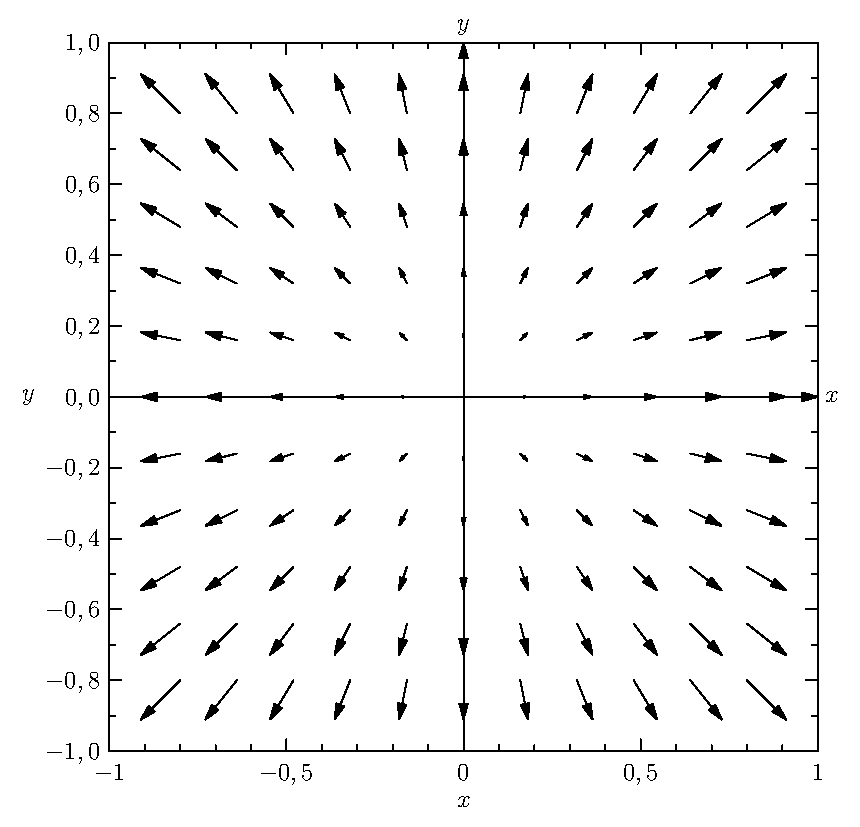
\includegraphics{cap_campos/figs/campo_radial}
%\caption{\label{campo_radial}Representação gráfica do campo $\vec{F}=\vec{r}$}
%\end{figure}
\end{ex}

\subsection*{Exercícios}
\begin{exer}
Mostre que $\vec{\nabla}\cdot\vec{r}=3$, $\vec{\nabla}\times\vec{r}=\vec{0}$ e $\vec{\nabla}r=\frac{1}{r}\vec{r}=\hat{r}$, sendo $\vec{r}(x,y,z)=x\vec{i}+y\vec{j}+z\vec{k}$.
\end{exer}
\begin{exer}\label{ex_grad_campo_central}
Dada a função escalar $f(r)$, onde $r=\|\vec{r}\|=\sqrt{x^2+y^2+z^2}$, use a regra da cadeia para mostrar que 
$$
\vec{\nabla}f(r)=\frac{f'(r)}{r}\vec{r}=f'(r)\hat{r}.
$$
Aplique essa fórmula para mostrar que $\vec{\nabla}r^n=nr^{n-2}\vec{r}.$
\end{exer}
\begin{exer}Use os resultados do exercício \ref{ex_grad_campo_central} para calcular $\vec{\nabla}f(r)$ para
\begin{itemize}
 \item[a)] $f(r)=r^3$.
 \item[b)] $f(r)=\ln(r)$.
 \item[c)] $f(r)=r^2e^{-r}$.
\end{itemize}
\end{exer}
\begin{resp}
\begin{itemize}
 \item[a)] $3r\vec{r}$.
 \item[b)] $\frac{\vec{r}}{r^2}$.
 \item[c)] $(2-r)e^{-r}\vec{r}$.
\end{itemize} 
\end{resp}
\begin{exer}
 Mostre que
 $$
 \vec{\nabla}^2f(r)=2\frac{f'(r)}{r}+f''(r),
 $$
 onde $r=\|\vec{r}\|=\sqrt{x^2+y^2+z^2}$. Utilize este resultado para mostrar que:
 \begin{itemize}
  \item[a)] $\vec{\nabla}^2\ln(r) =\frac{1}{r^2}$. 
  \item[b)] $\vec{\nabla}^2r^n =n(n+1)r^{n-2}$.
  \item[c)] $\vec{\nabla}^2\ln(r^2) =\frac{2}{r^2}$.
    \item[d)] $\vec{\nabla}^2\left(\frac{1}{r}\right) =0$.
 \end{itemize}
\end{exer}

\begin{exer}
 Uma partícula de massa $m$ e velocidade $\vec{v}$ é atraída para a origem por uma força central dada por $\vec{F}(\vec{r})=f(r)\hat{r}$. Mostre que o momento angular $\vec{L}=\vec{r}\times m\vec{v}$ é constante, isto é, $\frac{d\vec{L}}{dt}=\vec{0}$
\end{exer}
\begin{exer}
 Mostre que um campo central $\vec{F}(r)=f(r)\hat{r}$ é irrotacional.
\end{exer}


\section*{Exercícios finais}

\construirExer

\begin{exer}
  Um exercício.
\end{exer}
\begin{resp}
  Resposta curta do exercício.
\end{resp}
